\documentclass[problem]{mcs}

\begin{pcomments}
  \pcomment{PS_circuit_data_type}
  \pcomment{ARM draft 3/6/16}
\end{pcomments}

\pkeywords{
  circuit
  recursive
  structural_induction
  evaluate
}

\newcommand{\llist}[1]{{\mathop{\mathrm{list(#1)}}}}
\newcommand{\lcons}[2]{{\mathop{\mathrm{cons(#1,#2)}}}}
\newcommand{\cwout}{\textbf{O}}
\newcommand{\cwname}{\ensuremath{W}}
\newcommand{\bgat}{\ensuremath{\text{Gates}}}
\newcommand{\reccirc}{\text{DigCirc}}
\newcommand{\cwin}[1]{{\mathop{\mathrm{inputs(#1)}}}}
\newcommand{\ctern}[1]{{\mathop{\mathrm{internal(#1)}}}}
\newcommand{\cwirs}[1]{{\mathop{\mathrm{wires(#1)}}}}
\newcommand{\bools}{\set{\true, \false}}

\begin{problem}

We can explain in a simple and precise way how digital circuits work,
and gain the powerful proof method of structural induction to verify
their properties, by defining digital circuits as a recursive data
type $\reccirc$.  The definition is a little easier to state if all
the gates in the circuit take two inputs, so we will use the two-input
\QNOR\ gate rather than a one-input \QNOT, and let the set of gates be
\[
\bgat \eqdef \set{\QNOR, \QAND, \QOR, \QXOR}.
\]
A digital circuit will be a recursively defined list of \emph{gate
  connections} of the form $(x,y, G, I)$ where $G$ is a gate, $x$ and
$y$ are the input wires, and $I$ is the set of wires that the gate
output feeds into as illustrated in Figure~\ref{reccirc_contruct}.

\begin{center}
\begin{figure}%\inbook{[h]}
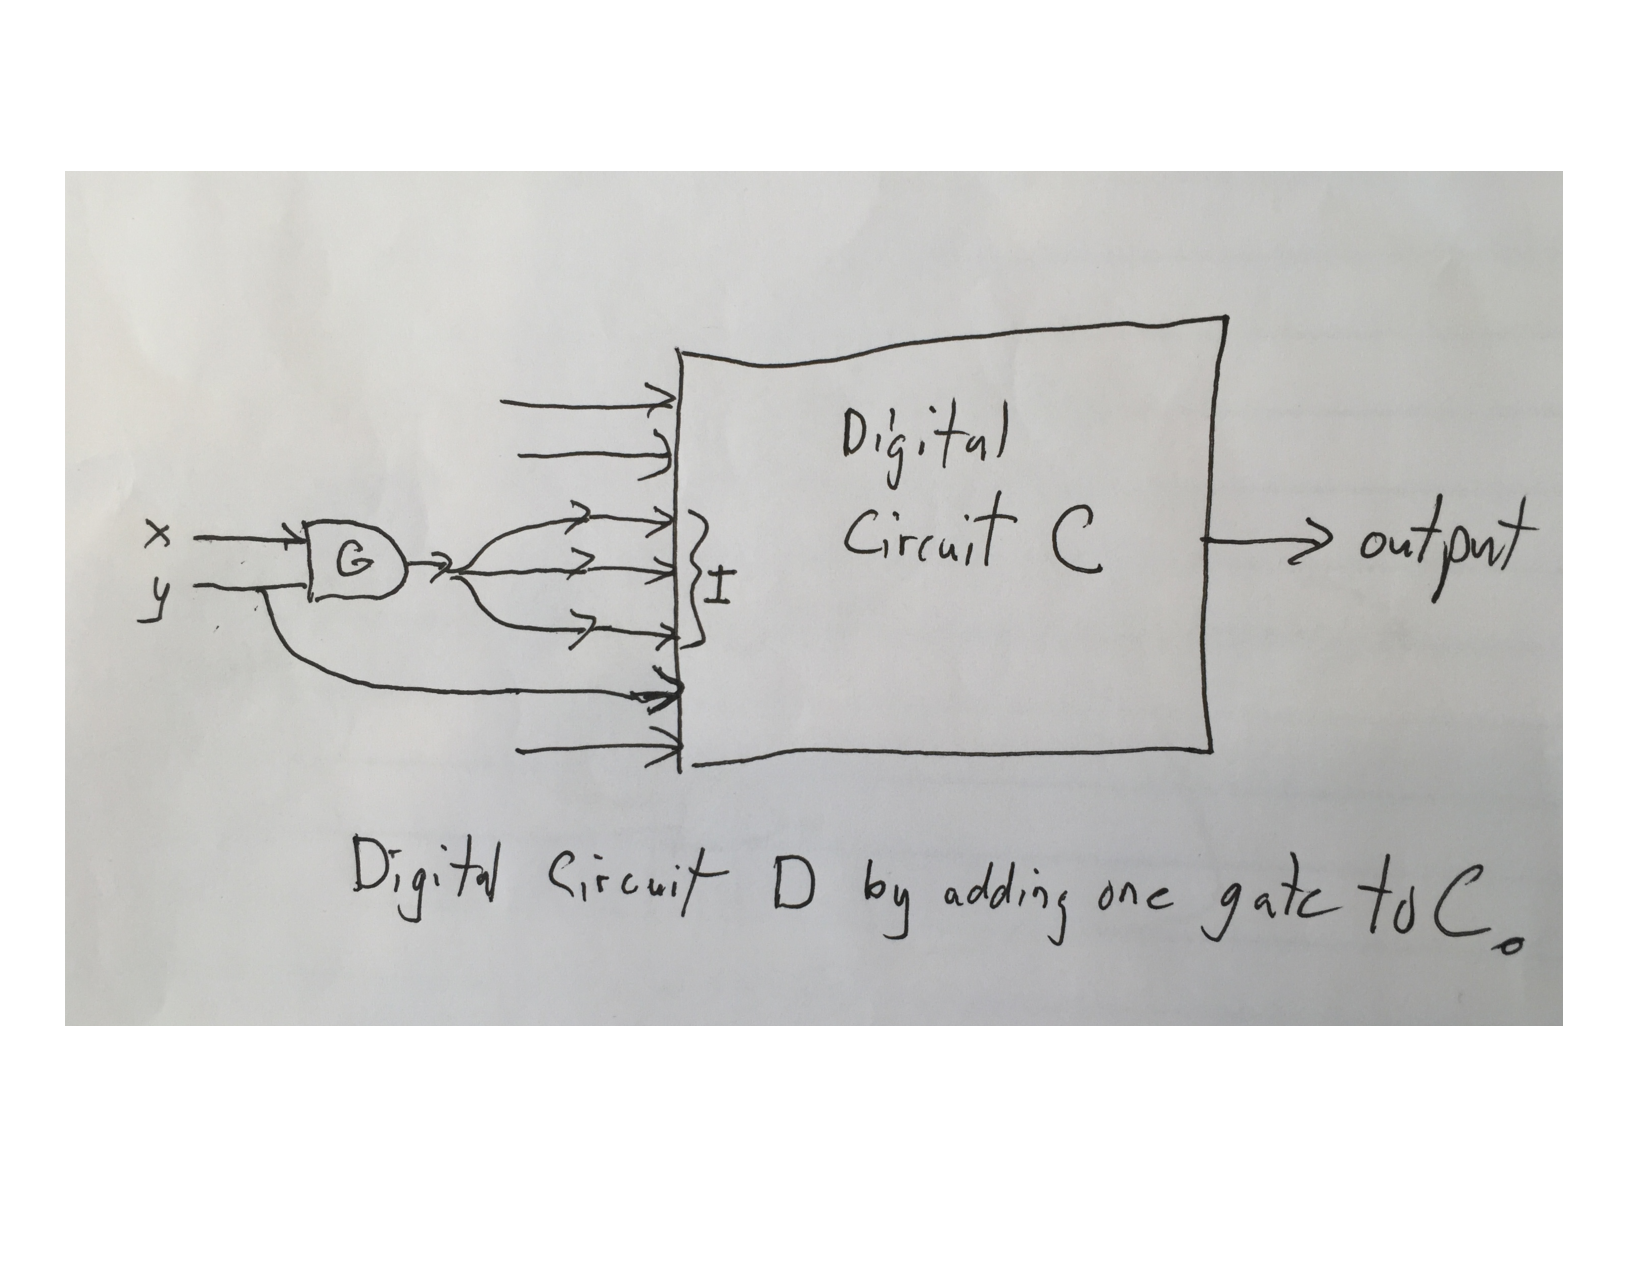
\includegraphics[width=5in]{circuit_data_type}
\caption{Digital Circuit Constructor Step}
\label{reccirc_contruct}
\end{figure}
\end{center}

Formally, we let $\cwname$ be a set $w_0,w_1,\dots$ whose elements are
called \emph{wires}, and $\cwout \notin \cwname$ be an object called
the \emph{output}.

\begin{definition*}
The set of digital circuit $\reccirc$, and their inputs and internal
wires, are defined recursively as follows:

\inductioncase{Base case:}
If $x, y \in \cwname$, then $C \in \reccirc$, where
\begin{align*}
C & = \llist{(x,y,G,\set{\cwout})}\text{ for some } G \in \bgat,\\
\cwin{C} &\eqdef \set{x,y},\\
\ctern{C} & \eqdef \emptyset.
\end{align*}

\inductioncase{Constructor cases:}
If
\begin{align*}
C & \in \reccirc,\\
I &\subseteq \cwin{C}, I \neq \emptyset,\\
x, y &\in \cwname - (I \union \ctern{C})
\end{align*}
then $D \in \reccirc$, where
\begin{align*}
D         & =  \lcons{(x,y, G, I)}{C} \text{ for some } G \in \bgat,\\
\cwin{D}  & \eqdef \set{x,y} \union (\cwin{C} - I),\\
\ctern{D} & \eqdef \ctern{C} \union I.
\end{align*}
\end{definition*}

\begin{editingnotes}
Sanity check: $\cwin{C} \intersect \ctern{C} = \emptyset$.
\end{editingnotes}

For any circuit $C$ define
\[
\cwirs{C} \eqdef \cwin{C} \union \ctern{C} \union \set{\cwout}.
\]
A \emph{wire assignment} for $C$ is a function
\[
\alpha: \cwirs{C}\to \bools
\]
such that for each gate connection $(x,y,G,I) \in C$,
\[
\alpha(i) = (\alpha(x)\ G\, \alpha(y))\text{ for all } i \in I.
\]

\bparts

\ppart\label{indetass} Define an \emph{environment} for $C$ to be a function $e:
\cwin{C} \to \bools$.  Prove that if two wire assignments for $C$ are
equal for each wire in $\cwin{C}$, then the wire assignments are
equal for all wires.
\eparts

\medskip

Part~\eqref{indetass} implies that for any environment $e$ for $C$,
there is a \emph{unique} wire assignment $\alpha_e$ such that
\[
\alpha_e(w) = e(w) \text{ for all } w \in \cwin{C}.
\]
So for any input environment $e$, the circuit computes a unique \emph{output}
\[
\meval{C}{e} \eqdef \alpha_e(\cwout).
\]

Now suppose $F$ is a propositional formula whose propositional
variables are the input wires \iffalse $\cwin{C}$ \fi of some circuit
$C$.  Then $C$ and $F$ are defined to be \emph{equivalent} iff
\[
\meval{C}{e} = \meval{F}{e}
\]
for all environments $e$ for $C$.

\bparts

\ppart Define a function $E(C)$ recursively on the definition of
circuit $C$, such that $E(C)$ is a propositional formula equivalent to
$C$.  Then verify the recursive definition by proving the equivalence
using structural induction.

\ppart Give examples where $E(C)$ is exponentially larger than $C$.

\eparts

\end{problem}

\endinput
